% !Mode:: "TeX:UTF-8"
%!TEX program  = xelatex

\documentclass{cumcmthesis}
%\documentclass[withoutpreface,bwprint]{cumcmthesis} %去掉封面与编号页

\usepackage{url}
\usepackage{amsmath}
\usepackage{amssymb}
\usepackage{gensymb}
\usepackage{graphicx}
\usepackage{float}
\title{高压油管的压力控制模型}
\tihao{C}
\baominghao{4321}
\schoolname{重庆邮电大学}
\membera{贺琛}
\memberb{谭淋}
\memberc{王菁精}
\supervisor{张清华}
\yearinput{2020}
\monthinput{09}
\dayinput{10}

\begin{document}

 \maketitle
 \begin{abstract}
高压燃油系统主要由高压油泵、高压油管、喷油嘴三部分构成,在高压系统的工作 原理下分析供油和喷油对高压油管腔内压力产生的影响。本文针对高压油管腔内压强的 控制问题,以液压油路模型为理论基础建立了完整的燃油系统模型。
\vspace{10pt}

{\heiti 针对问题一},首先基于液压油路模型的建模原理,建立高压油管压强的控制模型,得到高压油管流量与压强的关系式。问题一通过调节单向阀开启时长控制高压油管内的压强,利用{\heiti 残差平方和最小}得到初步的单向阀开启时长,再利用{\heiti 遗传优化算法}得到全局最优解:单向阀开启时长$T=0.28ms$时,高压油管内的压强稳定在100MPa;前 1.5s 单向阀开启时长$T=1.5s$,后0.5s开启时长$T=0.76ms$时 ,可使高压油管内压强经过约 2s 调整后稳定在 150MPa;当调整时长为 5s 时,前 3.1s 开启时长$T=10ms$,后 1.9s 开启时长$T=0.76ms$;当调整时长为 10s 时,前 8s 开启时长$T=2.8ms$,后2s开启时长$T=0.76ms$。
\vspace{10pt}

{\heiti 针对问题二},在问题一的高压油管模型的基础上进行改进,确定凸轮的角速度,使 高压油管内的压力尽量稳定在 100 MPa 左右,建立高压油泵模型分析供油量对高压油管 内压强的影响,建立喷油器模型分析出油量对高压油管内压强的影响,并结合问题一中 建立的{\heiti 高压油管压强控制模型},得到完整的燃油系统模型。结合问题一的求解思路,利 用 MATLAB 软件编程,通过迭代遍历的方法计算得到凸轮的角速度$\omega =0.0266rad/ms$时,油管内压力稳定在 100MPa 左右。
\vspace{10pt}

{\heiti 针对问题三}, 实质上是高压油管的压强控制问题。我们通过建立{\heiti 无约束非线性规划模型},在增加一个喷油嘴的情况下,从喷油器工作次数n、凸轮角速度 $\omega$、喷油器工作时差 $\tau$三个参数的角度,设计喷油和供油策略;在又安装一个单向减压阀的情况下,从 凸轮角速度$\omega$ 、单向减压阀每次的打开时间 $\mu$ 两个参数的角度,设计高压油泵和减压阀 的控制方案,保证高压油管内的压强稳定在 100MPa,求解思路与问题一类似,得出参 数的具体计算结果见正文 P18-P19,最后,利用多项拟合的方法对$\omega$-$\mu$ 最后,利用多项式拟合的方法对的变化曲线,得出拟合方程为:$\mu(\omega)=10540\omega^3-2145\omega^2+166.5\omega+26.05$ ,其拟合度为 99.73\%。
\vspace{10pt}

最后,将模型应用于 GDI 燃油系统研发。对模型进行客观评价,对模型的实用性进 行评估,并给出针对模型缺陷的改进方案。
\vspace{10pt}

\keywords{高压油管压强控制模型\quad  遗传算法\quad   无约束非线性规划模型 \quad  残差平方和 }
\end{abstract}


\section{问题重述}


\subsection{问题的背景}

燃油进入和喷出高压油管是许多燃油发动机工作的基础,某高压燃油系统的工作原 理下\textsuperscript{\cite{bib:one}}:燃油经过高压油泵从供油入口进入高压油管,再由喷油嘴喷出。燃油进入和 喷出的间歇性工作过程会导致高压油管内压力的变化,使得所喷出的燃油量出现偏差, 从而影响发动机的工作效率。 

其中高压油管系统作为发动机油路系统最为重要的组成部分之一,通过单向阀开关 控制供油时间的长短,单向阀每打开一次后就要关闭 10ms。油管与喷油器相连,喷油 器工作时从喷油嘴向外喷油,每秒工作 10 次,每次工作时喷油时间为 2.4ms。 

此外,高压油管处的燃油来自高压油泵的柱塞腔出口,凸轮驱动柱塞上下运动,喷 油由喷油嘴的针阀控制。其中柱塞运动到上止点位置时,柱塞腔残余容积为 20mm$^3$。柱 塞运动到下止点时,低压燃油会充满柱塞腔,压力为 0.5 MPa。针阀升程为 0 时,针阀 关闭;针阀升程大于 0 时,针阀开启,燃油向喷孔流动,通过喷孔喷出。 

\begin{figure}[htb] \centering 
	
	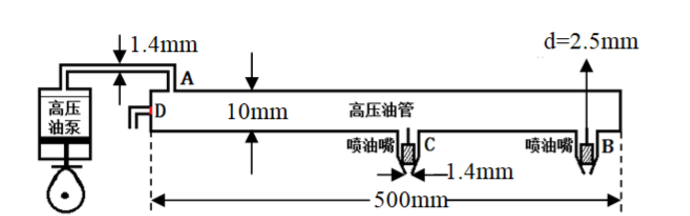
\includegraphics[width=12cm]{tu1.png} 
	
	\caption{高压油管工作过程示意图 } \label{fig:1} \end{figure} 
\subsection{问题的提出}
根据以上背景,以及给出的三个附件,需要解决以下问题: 

问题一:高压油泵在入口处提供的压力恒为 160 MPa,高压油管内的初始压力为 100 MPa。如果要将高压油管内的压力尽可能稳定在 100 MPa 左右,如何设置单向阀每次开 启的时长?如果要将高压油管内的压力从 100 MPa 增加到 150 MPa,且分别经过约 2 s、5 s和10 s 的调整过程后稳定在 150 MPa,单向阀开启的时长应如何调整?


问题二:在问题一中给出的喷油器工作次数、高压油管尺寸和初始压力下,确定凸 轮的角速度,使得高压油管内的压力尽量稳定在 100 MPa 左右。

问题三:在问题二的基础上,再增加一个喷油嘴,每个喷嘴喷油规律相同,喷油和 供油策略应如何调整?为了更有效地控制高压油管的压力,现计划安装一个单向减压阀。 单向减压阀出口为直径为 1.4mm 的圆,打开后高压油管内的燃油可以在压力下回流到 外部低压油路中,从而使得高压油管内燃油的压力减小。请给出高压油泵和减压阀的控 制方案。


\section{问题的分析}
\subsection{问题一的分析}
对于问题一,题目要求设计单向阀每次开启的时长,完成以下两个任务,任务一: 要求将高压油管内的压力稳定在 100MPa 左右;任务二:当高压油管内的压力从 100MPa 增加到 150MPa,要求经过规定时间的调整过程后稳定在 150MPa。通过单向阀开关控制 供油时间的长短即可实现泵油量的控制,最终实现高压油管内压力的调节。首先,我们 要使高压油管内的压力稳定在目标值,即表示在尽量小的周期内,保证压强越平稳越好, 其次根据题目可知喷油器每秒工作 10 次,即工作 1 次需要 100ms,由此我们将 100ms 作为高压油管的工作周期来研究工作过程中进油与出油对高压油管内压强的影响。问题 一分别从如下三种情形讨论高压油管的工作过程:(1)在 100ms 的工作周期内,进行先 出油后进油的操作来控制高压油管内压强的变化;(2)燃油同时从高压油泵流入高压油 管,又从高压油管进入到喷油嘴中喷出;(3)可能出现一个周期到另一个周期的过渡, 这时会出现预供油的情况,首先高压油泵提供燃油给高压油管,经过一段时间后,喷油 器才开始工作,喷油时间为 2.4ms,其中前两种情形造成压强在目标值之间的波动较大, 而第三种情形由于存在提前供油,使出油量与进油量能够保持相对平衡,管内压强波动 较小,然后将上述三种情形综合考虑,采用遗传算法求出最优的单向阀开启时长
\subsection{问题二的分析}
对于问题二,题目要求在问题一的基础上改变进油与出油的方式,在问题一中给出 的一些初始条件不变的情况下,确定凸轮的角速度,使得高压油管内的压力尽量稳定在 100 MPa 左右。与问题一类似,本问的实质也是压强控制问题,将自变量变为凸轮的角 速度,其中凸轮驱动柱塞上下运动,从而影响高压油泵流入高压油管的燃油流量。因为 本问变为由凸轮控制进油流量,由针阀控制出油流量,所以将本文划分为两部分进行讨 论:一方面分析高压油泵柱塞的压油过程对进油量的影响,建立高压油泵模型;另一方 面分析喷油器针阀的升程对出油量的影响,建立喷油器模型。然后在问题一中研究压强 与流量的工作基础上,写出高压油管内压强与流量的关系式,列出高压油管内压强的状 态变化方程,最后通过状态方程确定凸轮的角速度,使高压油管内的压力稳定在目标值 100MPa 左右。 
\subsection{问题三的分析}
对于问题三,题目要求在问题二的基础上增加一个喷油嘴后喷油与供油的策略,以 及再增加一个单向减压阀后,高压油泵和减压阀的控制方案。首先我们考虑增加一个喷 油器的情况,在该情况下如何供油与出油能够尽量控制高压油管内的压强在稳定值,其 中影响出油量的两个主要因素为:每个喷油嘴每秒喷油的次数以及两个喷油嘴第i次开始喷油的时间差值,因为喷油嘴 B、C 存在两种喷油状态,即要么两者同时喷油,要么 喷油时刻不同时;结合问题二考虑,影响进油量的主要因素为凸轮的转动角速度,所以 喷油与供油策略实质上就是确定喷油器工作次数、两个喷油嘴开始工作的时间差值以及 凸轮的角速度这三个参数。然后,我们考虑再增加一个单向减压阀的情况,设计高压油 泵和减压阀的控制方案,目标同样是控制高压油管内的压强保持稳定,对于高压油泵对 高压油管内压强的影响,仍然以油泵凸轮的转动角速度作为影响因素;对于加压阀对管 内压强的影响,则以单向减压阀每次打开时间作为影响因素,综上所述高压油泵和加压 阀的控制方案实质上就是确定凸轮角速度,以及所对应的单向减压阀开启时间两个参数。
\section{问题假设}
假设 1:整个油路系统的温度不变; 

假设 2:所有管路均为刚性,即忽略管路弹性; 

假设 3:高压油管系统正常工作过程中不会发生逆流; 

假设 4: 高压油管内的压力同步变化,即不考虑压力不均匀对喷射以及泵油的影响, 以及忽略压力波对系统的影响; 

假设 5:将凸轮的转动近似看作匀速转动过程,即凸轮转动过程中角速度不变。
\section{符号说明}
\begin{center}
\begin{tabular}{cc}
	\toprule[1.5pt]  %添加表格头部粗线
	符号&意义\\
	\midrule[1pt]  %添加表格中横线
	$E$&体积弹性模量\\
	$Q_{out}$&流出高压油管的油量\\
	$Q_{in}$&流入高压油管的油量\\
	$c$&流量系数\\
	$p'$&表示下一状态高压油管内的压强\\
	$p$&表示当前状态高压油管内的压强\\
	$A$&小孔出口的面积\\
	$T$&单向阀开启时长\\
	$\omega$&凸轮转动的角速度\\
	\bottomrule[1.5pt] %添加表格底部粗线
\end{tabular}
\end{center}

\section{模型的建立与求解}
\subsection{问题一模型的建立与求解}
发动机高压油路系统主要由高压油泵、高压油管、喷油嘴、压力调节阀、轨压传感器等部分组成\textsuperscript{\cite{bib:two}},本问要求控制高压油管内的压力使管内压强稳定在目标值 100MPa 或 150MPa,从问题分析中已知要在三种情形下讨论进出油导致的压强变化,根据高压油管的物理结构,结合液压油路的建模原,我们建立高压油管压强控制模型求出高压油管内压强状态的变化,再利用遗传优化算法计算出最优的单向阀开启时长。

\subsubsection{建模基本原理}
本问考虑到高压油管的物理结构,见图 2,从左端高压油泵的小孔 A 处进油到高压 油管,外接喷油器,燃油再从喷油嘴 B 处流出,然后结合液压油路部分建模原理\textsuperscript{\cite{bib:three}},我们得到高压油管模型的建模原理。
\begin{figure}[htb] \centering 
	
	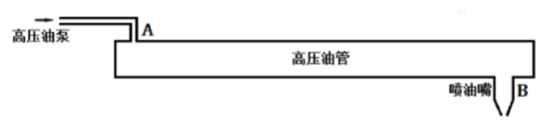
\includegraphics[width=10cm]{tu2.png} 
	
	\caption{高压油管示意图 } \label{fig:2} \end{figure} 

高压油管模型的建模原理如下:

1)设燃油的体积弹性模量为E ,则系统中燃油符合以下液体压缩模量公式:
\begin{equation}
E=\frac{-dp}{dV/V}=\frac{dp}{d\rho/\rho}\label{eq:1}
\end{equation} 

式(\ref{eq:2})中高压油管内燃油体积为V ,其中 p 为燃油压强, 为燃油密度,弹性模 量E与压力的关系由附件 3 可得。 由于固定燃油质量不发生变化,燃油密度与体积有关,所以可以将式\ref{eq:1}进行变换可得: 
\begin{equation}
\frac{dp}{dt}=-\frac{E}{V}\cdot\frac{dV}{dt}\label{eq:2}
\end{equation} 

2)利用流量代替燃油体积的变化率\textsuperscript{\cite{bib:four}}可得: 
\begin{equation}
\frac{dV}{dt}=\frac{dV_{0}}{dt}-q_{in}+q_{out}\label{eq:3}
\end{equation}


式(\ref{eq:1})中 $V_{0}$ 表示高压油管的容量,其中$\frac{dV_{0}}{dt}$
为容积的变化率,$q_{in}$为进入油管的流体的流量,$q^{out}$ 为流出油管的流体的流量。结合式(\ref{eq:2})得高压油管内部压力为: 
\begin{equation}
\frac{dp}{dt}=-\frac{E}{V}\cdot\left(\frac{dV_{0}}{dt}-q_{in}+q^{out}\right)\label{eq:4}
\end{equation}

 3)单位时间流过小孔的燃油量的计算公式\textsuperscript{\cite{bib:five}}为:
 \begin{equation}
 Q=sgn(\Delta p)\cdot C\cdot A\cdot\sqrt\frac{{2\lvert \Delta p \rvert}}{\rho}\label{eq:5}
 \end{equation}
其中C =0.85为流量系数,A为小孔的面积,$\Delta$p为小孔两边的压力差,$\rho$为高压侧
燃油的密度。sgn 为阶跃函数: 
 \begin{equation*}
sgn(\Delta p)=\begin{cases}
1\\
0\\
-1
\end{cases}
\end{equation*}

燃油的压力变化量与密度变化量成正比,比例系数为$\frac{E}{\rho}$
,则燃油的密度为 
 \begin{equation*}
\begin{cases}
\Delta p=\frac{E}{\rho}\cdot\left(\rho'-\rho\right)\\
\rho'=\frac{\left(\Delta \rho+E\right)\cdot\rho}{E}
\end{cases}
\end{equation*}


由假设 3 可知,忽略高压油管工作过程中发生逆流的情况,取$sgn(\Delta \rho)=1$由此流量公式(\ref{eq:5})变换为:
 \begin{equation}
 Q=C\cdot A\cdot\sqrt\frac{{2\lvert \Delta p \rvert}}{\rho}\label{eq:6}
 \end{equation}

结合公式(\ref{eq:4})、(\ref{eq:6})可得流出油管的油量$Q_{out}$计算公式与流入油管的油量$Q_{in}$计算公式为: 
\begin{equation}
	\begin{cases}
	Q_{in}=c_{in}\cdot A_{in}\cdot \sqrt{\frac{2\lvert \Delta \rho \rvert}{\rho}}\cdot t \\
	Q_{out}=x\cdot t
	\end{cases}\label{eq:7}
\end{equation}

公式(\ref{eq:7})中 $c_{in}$为高压油管进油入口处流量系数,表示高压油泵出油口孔径形状对 燃油流量的影响, $A_{in}$为高压油泵出口截面积,x表示喷油嘴的喷油速率。由于高压油管 工作过程中仅从喷油器喷出燃油,所以油管的出油量为喷油速率与时间的乘积;而进油 量则来自高压油泵的供给。

\subsubsection{高压油管压强控制模型的建立}
对于高压油管而言,其进油量为高压油泵供给高压油管的油量,由单向阀开启时间 的长短控制,出油量为高压油管供给喷油器的油量,而高压油管的体积没有变化,所以
建模原理式$\left(\ref{eq:4}\right)$ 中$\frac{dV_{0}}{dt}=0$
,基于上述建模原理的分析,我们以出油总压强与进油总压
强达到平衡作为约束条件,建立下面三种情形下高压油管的压强控制模型。

{\heiti 情形一:先出油,后供油} 

根据题目可知喷油器每秒工作 10 次,每次工作时间为 2.4ms,所以以 100ms 作为 高压油管的工作周期,在这个周期内有 2.4ms 从喷油嘴喷出燃油,在情形一中,假设从零时刻起开始出油,而供油有两种情况:一方面在经过 $\Delta t$时间后高压油管开始进油,$\Delta t<2.4 ms$ ;另一方面当出油结束后高压油管才开始进油。 

首先,考虑情形 1.1(见图\ref{fig:3})时高压油管内压强状态的变化。

\begin{figure}[htb] \centering 
	
	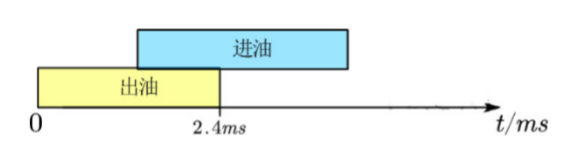
\includegraphics[width=10cm]{tu3.png} 
	
	\caption{情形 1.1 示意图 } \label{fig:3} \end{figure} 

1)当 $t\le\Delta t \le2.4ms$ 时,仅有从高压油管流入喷油器的出油流量,即出油量增多;

 2)当 $\Delta t\leq t\le 2.4ms $时,既有从高压油泵流入高压油管的进油流量,又有从高压油 管流入喷油器的出油流量,则高压油管内的压力变化与两者都有关; 
 
 3)当$2.4ms\leq t \le100ms$时,只有从高压油泵流入高压油管的进油流量,即进油量增多。 
 
 综上,列出情形 1.1 下高压油管的压强控制模型为: 

  \begin{equation}
 \begin{cases}
 p'=\frac{\left({V_{r}-Q_{out}}\right) \times p}{V_{r}},&t\le \Delta t \le 2.4ms\\
 p'=\frac{\left[ V_{r}-Q_{out}+Q_{in} \right] \times p}{V_{r}},&\Delta t \leq t \le 2.4ms\\
 p'=\frac{\left( V_{r}+Q'_{in} \right)\times p}{V_{r}},&2.4ms\leq t \le 100ms 
 \end{cases}\label{eq:8}
 \end{equation}
 
公式中(\ref{eq:8}),$p'$表示下一状态高压油管内的压强,它会随着高压油管内的进出油量的变化而发生改变,$V_{r}$ 为高压油管的体积,开始时高压油管的出油量$Q_{out}$ 大于进油量$Q_{in}$ ,随着高压油泵不断为高压油管提供燃油,出油量与进油量趋于平衡,管内压强也 从下降趋势逐渐上升到 100MPa 左右并使其保持稳定。 


其次,考虑情形 1.2(见图\ref{fig:4})时高压油管内压强状态的变化。
\begin{figure}[htb] \centering 
	
	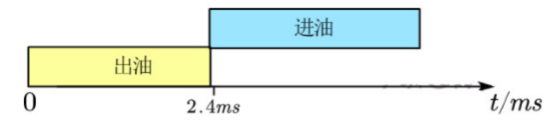
\includegraphics[width=10cm]{tu4.png} 
	
	\caption{情形 1.2 示意图 } \label{fig:4} \end{figure} 

1)当 $t\le 2.4ms$时,高压油管仅从喷油器喷出油,出油量增加; 

2)当$2.4ms\leq t\le 100ms$时,高压油管只进油不喷出油,且每进油一次后单向阀关闭 10ms,喷油量增加。 

同样列出情形 1.2 下高压油管的压强控制模型,开始时出油量 $Q_{out}$大于进油量$Q_{in}$ , 然后随着燃油的进入,管内压强逐渐上升到 100MPa, 
\begin{equation}
\begin{cases}
p'=\frac{\left(V_{r}-Q_{out}\right)\times p}{V_{r}},&t\le 2.4ms\\
p'=\frac{\left(V_{r}+Q'_{out}\right)\times p}{V_{r}},&2.4ms\leq t\le 100ms
\end{cases}\label{eq:9}
\end{equation}


{\heiti 情形二:同时出油和供油}

在情形二中,设从零时刻起出油与进油同时进行,并且在 2.4ms 后,周期内不再喷 油,但还存在从高压油泵供给高压油管燃油的过程,下面考虑情形 2(见图 \ref{fig:5})时高压 油管内压强状态的变化。 
\begin{figure}[htb] \centering 
	
	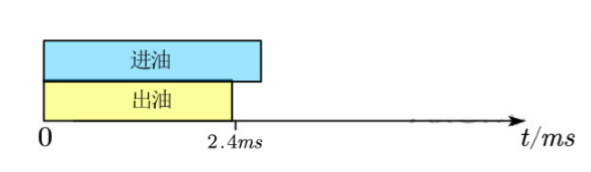
\includegraphics[width=10cm]{tu5.png} 
	
	\caption{情形2示意图 } \label{fig:5} \end{figure} 

1)$t\le2.4ms$ 时,出油与供油操作同时进行,此时进油量上升,出油量增加; 

2)当$2.4ms\leq t\le100ms$时,存在高压油泵进入高压油管的燃油流量,进油量继续增 加,但出油量不会发生变化。 综上,列出情形 2 下高压油管的压强控制模型为:
\begin{equation}
\begin{cases}
p'=\frac{\left[V_{r}-Q_{out}+Q_{in}\right]\times p}{V_{r}},&t\le 2.4ms\\
p'=\frac{\left(V_{r}+Q'_{in}\right)\times p}{V_{r}},&2.4ms\leq t\le 100ms
\end{cases}\label{eq:10}
\end{equation}

虽然在情形二中进油与出油操作同时进行,但由于高压油泵腔内压强与高压油管强 内压强之差小于压强高压油管强内压强与喷油器外压强之差,所以进油总压强小于出油 总压强,若想使压强稳定在目标值,则仍需继续进油操作。

{\heiti 情形三:预供油,后出油} 

在情形三中,通过高压油泵进入高压油管的燃油流量,经过$\Delta t'$时间后,喷油器开 始工作,从高压油管流出燃油流量,在这一情形下,要使高压油管的压强稳定在目标值 可能出现以下三种情形:Ⅰ.在高压油管的工作过程中,经过 2.4ms 出油结束后,还需再 进油,因为此时出油量 $Q_{out}$ 大于进油量 $Q_{in}$ ;Ⅱ.进油操作和出油操作同时结束,出油量 $Q_{out}$与进油量 $Q_{in}$达到平衡;Ⅲ.进油操作结束后,喷油器还在工作,因为此时出油量 $Q_{out}$小于进油量 $Q_{out}$ 。 

下面考虑情形 3(见图\ref{fig:6})时高压油管内压强状态的变化。
\begin{figure}[htb] \centering 
	
	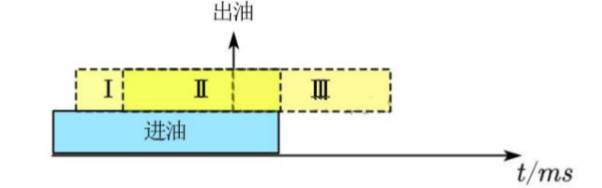
\includegraphics[width=10cm]{tu6.png} 
	
	\caption{情形3示意图 } \label{fig:6} \end{figure} 

1)当$t\le \Delta t'$时,只有高压油泵流入高压油管的进油流量,进油量增加; 

2)当$t\le \Delta t'+2.4ms$时,既存在进油又存在出油,进油量与出油量都增加; 

3)当$\Delta t'+ 2.4ms \leq t \le 100ms$时,与管内油量变化与 1)相同。 综上,列出情形 3 下高压油管的压强控制模型为:
\begin{equation}
\begin{cases}
p'=\frac{\left(V_{r}+Q'_{in}\right)\times p}{V_{r}},&t\le \Delta t' \quad or\quad  \Delta t'+2.4ms \leq t \le 100ms\\
p'=\frac{\left[V_{r}-Q_{out}+Q_{in}\right] \times p}{V_{r}},&\Delta t' \leq t \le \Delta t' +2.4ms
\end{cases}\label{eq:11}
\end{equation}

情形 3 相对于情形 1 和情形 2,出油量与进油量造成高压油管内压强的波动更小, 在模型求解的过程中我们需要将三种情形结合考虑,计算出最优的单向阀开启时长。

\subsubsection{高压油管压强控制模型的求解与分析}
本问要求解单向阀的开启时长使得压强稳定在目标值,并且根据题目可知单向阀每 打开一次后就要关闭 10ms,从上述的模型建立中我们知高压油管的工作周期为 100ms, 现需确定单向阀开启时长,结合公式求出高压油管内的压强, 并使得在该时长下的压强能够稳定在目标值。

 模型求解的步骤如下,其求解思路流程图见图\ref{fig:7}: 
 
 \begin{figure}[htb] \centering 
 	
 	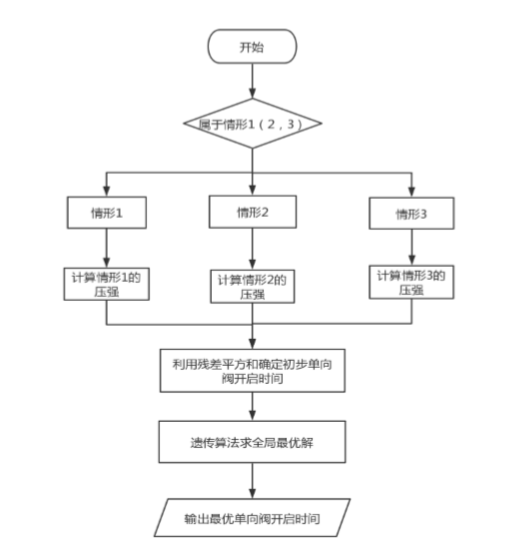
\includegraphics[width=12cm]{tu7.png} 
 	
 	\caption{高压油管压强控制模型的求解思路流程图} \label{fig:7} \end{figure} 
 
 Step1: 确定单向阀开启时长的上限; 根据题目给出的喷油速率示意图,能够求出在一个工作周期内的总喷油量,设周期 内单(\ref{eq:8}),(\ref{eq:9}),(\ref{eq:10}),(\ref{eq:11})向阀开启时长为T 时,出油量 $Q_{out}$ 等于进油量 $Q_{in}$ ,则单向阀开启时长的范围为0$\sim$ T 。
设总出油量为 $Q'_{out}$ ,确定单向阀开启时长T 为: 

\begin{equation}
Q'_{out}=q_{in}\cdot T\label{eq:12}
\end{equation}

\begin{equation*}
  \text{即}\quad\frac{\left(240+200\right)\times 20}{2}=15.5\times T
\end{equation*}

\begin{equation*}
T=2.83ms
\end{equation*}

Step2: 在0$\sim$ T 的范围内随机选定单向阀开时长,利用公式(\ref{eq:8}),(\ref{eq:9}),(\ref{eq:10}),(\ref{eq:11}) 求出高压油管内的压强;

Step3:为了使高温油管内的压强稳定在目标值$\bar{p}$,则 压强$\hat{p_{t}}$与预期目标压强的差值 的绝对值要最小,本文引入残差平方和的概念作为评定差值最小的标准,求得使残差平方和最小的单向阀开启时长,初步确定单向阀开启时长; 
\begin{equation}
min=\sum_{t=0.01}^{T}e_{t}^{2}=\sum_{t=0.01}^{T}\left(\hat{p}_{t}-\tilde{p}\right)^{2}\label{eq:13}
\end{equation}

式(\ref{eq:13})中我们以$dt=0.01ms$作为迭代步长,每隔 0.01ms 计算压强值。 

Step4: 利用遗传优化算法,跳出局部最优解,求得全局最优解,最终确定单向阀时 长。 

根据上述求解步骤,利用 MATLAB 软件编程计算出任务一的结果如下,并且画出 残差平方和随单向阀开启时长的变化图:

 \begin{figure}[htb] \centering 
	
	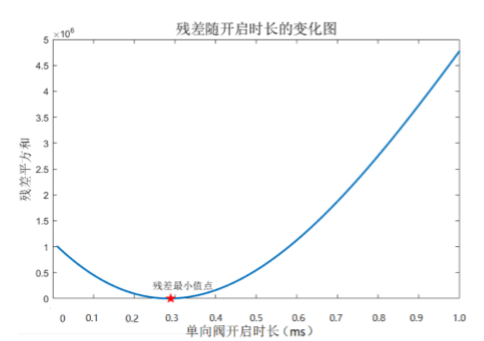
\includegraphics[width=10cm]{tu8.png} 
	
	\caption{残差平方和变化图} \label{fig:8} \end{figure}  

\begin{table}[!htbp]
	\caption{压力稳定在 100MPa 时单向阀的开启时长}\label{tab001} \centering
	\begin{tabular}{cc}
		\toprule[1.7pt]
		目标压力稳定值 & 单向阀每次开启时长 \\
		\midrule[1pt]
		100MPa& 0.28ms \\
	
		\bottomrule[1.7pt]
	\end{tabular}\label{tab:1}
\end{table}

观察图\ref{fig:8},发现当单向阀开启时间接近 0.3ms 时,残差平方和最小,即压强与预期 目标压强的差值的绝对值最小。再利用遗传优化算法求解全局最优解为 0.28ms,分析表\ref{tab:1},得出单向阀开启时长为 0.28ms 时,可以使高压油管内的压力尽可能稳定在 100MPa 左右,下面的压力变化图\ref{fig:9}能够更直观地观察出开启时长为 0.28ms 时,高压油管内的 压力在 100MPa 左右波动,并且波动不大。 

\begin{figure}[htb] \centering 
	
	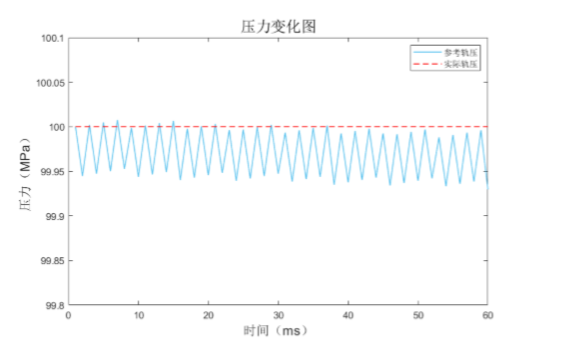
\includegraphics[width=10cm]{tu9.png} 
	
	\caption{高压油管内的压力变化图} \label{fig:8} \end{figure}  


同样根据上述求解步骤,利用 MATLAB 软件编程求解任务二,求得单向阀开启时 长能够使高压油管内的压力从 100MPa 增加到 150MPa,经过 2s、5s 和 10s 的调整后稳 定在 150MPa。任务二与任务一的不同之处在于,任务二中高压油管内的压力会先有一 个上升过程,在经过短时间调整后,再平稳在目标值 150MPa,下面表 2 展示的是任务 二的计算结果:

\begin{table}[!htbp]
	\caption{压力稳定在 150MPa 时单向阀的开启时长 }\label{tab002} \centering
	\begin{tabular}{cc}
		\toprule[1.5pt]
		调整时间(秒)& 调整过程 \\
		\midrule[1pt]
		\multirow{2}*{2}&{$t\le 1.5s$时,T=1.5s} \\
						~&{$1.5s\leq t \le 2s$时,T=0.76ms}\\
		\multirow{2}*{5}&{$t\le 3.1s$时,T=10ms}\\
						~&{$t\le 8s$时,T=2.8ms}\\
		\multirow{2}*{10}&{$t\le 8s$时,T=2.8ms}\\
						~&{$8s\leq t \le 10s$时,T=0.76ms}\\
		
		\bottomrule[1.5pt]
	\end{tabular}\label{tab:2}
\end{table}

分析表\ref{tab:2},当调整时间t=2s:$t\le1.5s$ 时设置单向阀开启时长T=1.5s,使油管内压 强上升,$1.5s\leq t\leq 2s$时设置单向阀开启时长T=0.76ms,使压强稳定在 150MPa;当调 整时间$t=5s$时设置单向阀开启时长T=10ms,使油管内压强上升,$3.1s\leq t\leq 5s$ 时设置单向阀开启时长T=0.76ms,使压强稳定在 150MPa;当调整时间t=10s:$t\le8s$时设置单向阀开启时长T=2.8ms,使油管内压强上升$8s\leq t \leq 10s$时设置单向阀开启时 长T=0.76ms,使压强稳定在 150MPa。下面图\ref{fig:10}展示了三个不同的调整时间下压力随 时间的变化图: 
\begin{figure}[htb] \centering 
	
	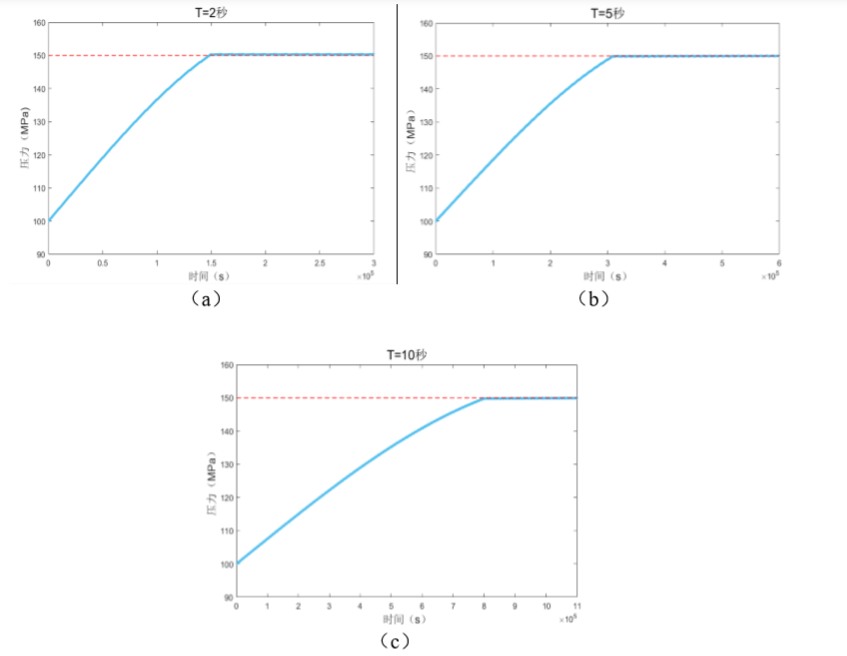
\includegraphics[width=16cm]{tu10.png} 
	
	\caption{不同的调整时间下的压力变化图} \label{fig:10} \end{figure}  

\subsection{问题二模型的建立、求解与分析}
问题二要建立完整的燃油系统模型,整个模型包括高压油泵模型、高压油管模型、 喷油器模型三部分,其中高压油管模型可利用问题一中的压强控制模型,而高压油泵模 型和喷油器模型分别控制高压油管内的进油量与出油量,与问题一求解思路类似,综合 三模型求得当油管内压强控制在预期目标值时,最优的凸轮角速度值,在求解凸轮角速 度时,重点分析高压油泵模型中凸轮极角与各参数的关系,由极角推出角速度的值。 

\subsubsection{高压油泵模型的建立}
问题二从高压油泵流入高压油管的流量是由高压油泵凸轮的驱动来决定的\textsuperscript{\cite{bib:six}},不能 直接通过控制单向阀的开关进油,而是凸轮驱动柱塞上下运动\textsuperscript{\cite{bib:seven}},油,当柱塞腔内的压力大于高压油管内的压力时,单向阀才开启进油,所以本问高压油 泵内的压强会随着凸轮的转动发生变化。 现在我们需要分析在改变进油方式后,高压油管的进油量$Q_{in}$,结合公式\ref{eq:6}可得: 
\begin{equation*}
Q'_{in}=c_{in}\cdot A_{in}\cdot \sqrt{\frac {2 \lvert \Delta p \rvert}{\rho}}\cdot t
\end{equation*}

 与问题一不同,问题二高压油泵内的压强不为定值,它会随着凸轮的转动发生变化, 影响进油量,所以我们要考虑凸轮转动对油泵内压强的影响\textsuperscript{\cite{bib:eight}} ,凸轮的部分转动过程见 图\ref{fig:11}。
 
 \begin{figure}[htb] \centering 
 	
 	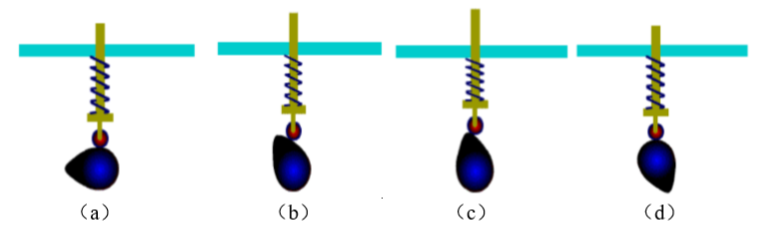
\includegraphics[width=16cm]{tu11.png} 
 	
 	\caption{凸轮模拟转动过程} \label{fig:11}
  \end{figure}  
  
 
 首先,根据附件 1 凸轮边缘曲线与角度的关系,发现凸轮在转动过程中,它的极径 随着角度的增加呈现先下降后升高的趋势,并且极径的变化代表高压油泵内柱塞的升程 变化,柱塞上升泵内压强就会升高。从题目知柱塞运动到下止点时,低压燃油的压力为 0.5MPa,由附件 1 得此时$\rho_{min}=2.413mm$ ;当极径最大时$\rho_{max}=7.239mm$,此时柱塞运动 到上止点,泵内压力最大,由最大最小极径,可以得到下止点与上止点间的距离:
 \begin{equation}
 l=\rho_{max}-\rho_{min}=7.239mm-2.413mm=4.826mm\label{eq:14}
 \end{equation}
此外,根据已知当柱塞运动到上止点位置时,还有 320mm 的残余容积$V_{c}$ ,并且已知 柱塞腔内直径为 5mm,所以可以求得残余容积部分的高度,S 为柱塞腔的底面积: 
\begin{equation}
h_{l}=\frac{V_{c}}{S}=\frac{20}{\pi \cdot 2.5^{2}}\label{eq:15}
\end{equation}


结合式(\ref{eq:14})、(\ref{eq:15})可得下止点到高压油泵顶端的距离为: $H=l+h_{l}$其次,由参考文献\textsuperscript{\cite{bib:one}}知燃油的体积压缩系数k 为: 
\begin{equation}
k=\frac{1}{E}=-\frac{dv/V}{dp}\label{eq:16}
\end{equation}

式(\ref{eq:16})中V 表示柱塞腔内的总体积,E 为弹性模量,从该式可以看出压缩系数是 弹性模量的倒数,其中 
\begin{equation}
\frac{dv}{V}={\Delta h}{H}={\Delta h}{l+h_{l}}\label{eq:17}
\end{equation}
式(\ref{eq:17})中$\Delta h$为凸轮每转动 0.01rad 极径的变化量,即柱塞升程的改变量,说明极 径变化量是关于极角的函数。 结合式(\ref{eq:16})、(\ref{eq:17})可推导出高压油泵内压强的状态方程为:
\begin{equation}
p'_{g}=\frac{-E\cdot \Delta h \left(\theta \right)}{l+h_{l}}+p_{g}\label{eq:18}
\end{equation}
式(\ref{eq:18})中$p'_{g}$表示凸轮转动 0.01rad 后相对于转动前油泵内的压强 $p_{g}$ ,当前高压油 泵内的压强,可以看出 $p'_{g}$是一个与凸轮极角 $\theta$有关的函数。 

根据题目要求,只有当高压油泵内的压大于高压油管内的压强时,燃油才会从油 泵流入油管,我们已知油管内的初始压力$p_{0}=100MPa$,所以当高压油泵内压强大于 100MPa 时才会使单向阀打开向管内压油,利用公式(\ref{eq:18})计算出当高压油泵内压强为 100MPa 时,凸轮的极角$\theta=2.61rad\;or\; \theta=3.67rad$,由此可得凸轮转动过程中极角的范 围属于0$\sim$2.61rad 或3.67$\sim$6.27rad 时,燃油才从高压油泵流入高压油管,图\ref{fig:12}展示了极径随极角的变化图。
 \begin{figure}[htb] \centering 
	
	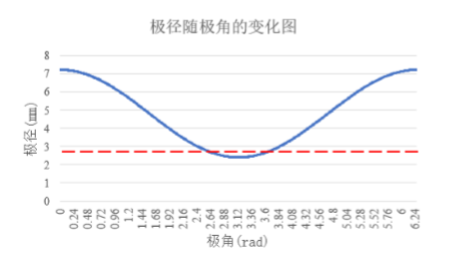
\includegraphics[width=10cm]{tu12.png} 
	
	\caption{极径随极角的变化图 } \label{fig:12}
\end{figure}  

综上可得,从高压油泵流入高压油管内的燃油量为: 
\begin{equation}
Q'_{in}=c_{in}\cdot A_{in}\cdot \sqrt{\frac{2\rvert p'_{g}\left(\theta \right)-p\rvert}{p}}\cdot t,\theta \in \left(0\sim 2.61rad\right)\cap \left(3.67\sim 6.27rad\right)\label{eq:19}
\end{equation}

\subsubsection{喷油器模型的建立}
根据题目知喷油器工作次数不变,即喷油器每秒钟工作 10 次,仍可划分为工作一 次需要 100ms,此外,本问喷油器系统不仅包含喷油嘴\textsuperscript{\cite{bib:nine}},还有控制喷油流量的针阀组 成,针阀升程为 0 时,针阀关闭;针阀升程大于 0 时,针阀开启,燃油向喷孔流动,通 过喷孔喷出,通过附件 2 可知一个喷油周期内针阀升程与时间的关系,画出针阀的上升 高度随时间的变化图,见图\ref{fig:13}。 

 \begin{figure}[H] \centering 
	
	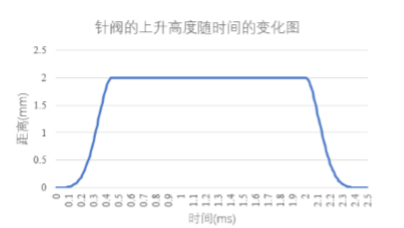
\includegraphics[width=8cm]{tu13.png} 
	
	\caption{针阀的上升高度随时间的变化图} \label{fig:13}
\end{figure}  

根据喷油器的物理结构见图\ref{fig:14}\textsuperscript{\cite{bib:ten}},分析在带有针阀的条件下,喷油嘴的出油量$Q_{out}$。

 \begin{figure}[htb] \centering 
	
	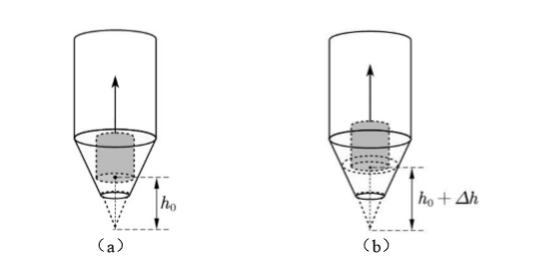
\includegraphics[width=12cm]{tu14.png} 
	
	\caption{喷油器的物理结构} \label{fig:14}
\end{figure}  


我们将通过喷油嘴与针阀之间的缝隙的燃油流量作为出油量,结合公式(\ref{eq:6})可以 得到喷油嘴的出油量为: 
\begin{equation}
Q'_{out}=c_{out}\cdot S_{crack}\cdot\sqrt{\frac{2\Delta p}{\rho}}\cdot t\label{eq:20}
\end{equation}

式(\ref{eq:20})中$S_{crack}$为缝隙的面积,是同一水平面上针阀底面积$S_{z}$与喷油嘴横截面积$S_{j}$的差值, 
\begin{equation}
\begin{cases}
S_{crack}=S_{j}-S_{z}\\
S_{z}=1.25^{2}\cdot \pi
\end{cases}\label{eq:21}
\end{equation}

其中我们已知针阀的直径为 2.5mm,将针阀的底面看作一个圆可求得针阀的底面积 为 $1.25^{2}\cdot\pi$,喷油嘴横截面积$S_{j}$的求法较为复杂,如下分析\begin{equation}
h_{0}=\frac{r_{z}}{\tan 9\degree}=\frac{1.25mm}{\tan 9\degree}\label{eq:22}
\end{equation}
 由附件 2 针阀升程与时间的关系,可知当针阀上升$\Delta h$后,在 $h_{0}+\Delta h$ 的高度处喷油 嘴的横截面积$S_{j}$为:
 
 可以求得缝隙的面积$S_{crack}$ 为:
 \begin{equation}
 	\begin{cases}
 	R=\left(h_{0}+\Delta h\right)\cdot\tan 9\degree\\
 	S_{j}=\pi\cdot R^{2}
 	\end{cases}\label{eq:23}
 \end{equation}
 
 通过公式(\ref{eq:22}),(\ref{eq:23})可以求得缝隙的面积$S_{crack}$为: 
 \begin{equation}
 S_{crack}=\pi\cdot\Delta h\cdot \left(\tan 9\degree\right)^{2}\cdot\left(\Delta h+2h_{0}\right)\label{eq:24}
 \end{equation}
 
 综上,可以将公式(\ref{eq:20})变换为:
 \begin{equation}
 Q'_{out}=c_{out}\cdot \left[\pi \cdot \Delta h \cdot \left(\tan 9\degree \right)^{2}\cdot \left(\Delta h +2h_{0}\right)\right]\cdot\sqrt{\frac{2p}{\rho}}\cdot t\label{eq:25}
 \end{equation}
\subsubsection{燃油系统模型的求解与分析}
在问题一高压油管压强控制模型的基础上,结合公式(\ref{eq:19})、(\ref{eq:25})型为\textsuperscript{\cite{bib:two}}: 
\begin{equation}
\begin{cases}
\begin{cases}
Q'_{in}=c_{in}\cdot A_{in} \cdot \sqrt{\frac {2\lvert p'_{g}\left(\theta\right)-p\rvert}{\rho}}\cdot t\\
\theta=\omega\cdot dt\quad\theta\in\left(0\sim2.61rad\right)\cup\left(3.67\sim6.27rad\right)\\
Q'_{out}=c_{out}\cdot\left[\pi\cdot\Delta h \cdot\left(\tan 9\degree\right)^{2}\cdot\left(\Delta h +2h_{0}\right)\right]\cdot\sqrt{\frac {2p}{\rho}}\cdot t\\
\end{cases}
\\
p'=\begin{cases}
\frac{\left(V_{r}-Q'_{out}\right)\times p}{V_{r}}\\
\frac{\left[V_{r}-Q'_{out}+Q'{in}\right]\times p}{V_{r}}\\
\frac{\left(V_{r}+Q'_{in}\right)\times p}{V_{r}}
\end{cases}
\end{cases}\label{eq:26}
\end{equation}
根据题目要求,本问要确定凸轮的角速度,使得高压油管内的压力尽量稳定在 100MPa 左右,由于高压油泵模型中的各个参数都与凸轮极角有关,为确定角速度与这 些参数的关系,通过公式$\theta=\omega\cdot dt$找到凸轮极角与角速度的关系式,求出角速度$\omega$。 

此问与问题一求解思路类似见图 7,通过燃油系统模型,利用 MATLAB 软件编程, 逐步迭代遍历求出使得高压油管内的压力尽量稳定在100MPa左右的最优凸轮角速度为:
\begin{table}[!htbp]
	\caption{最优凸轮角速度 }\label{tab003} \centering
	\begin{tabular}{cc}
		\toprule[1.7pt]
		目标压力稳定值(MPa) &凸轮角速度(rad/ms)\\
				\midrule[1pt]
		100& 0.0266 \\
		
		\bottomrule[1.7pt]
	\end{tabular}\label{tab:3}
\end{table}

\subsection{问题三模型的建立、求解与分析}
\subsubsection{喷油和供油策略模型的建立 }
从问题分析可知,影响出油量的有两个因素为:(1)B、C 喷油嘴,每个喷油器每 秒钟喷油的次数n,每次工作\textsuperscript{\cite{bib:one}}时喷油时间由附件 2 知为 2.45ms;( 2)两个喷油器每次 开始喷油时刻的时间差$\tau$。影响进油量(供油量)的主要因素为:凸轮转动的角速度$\omega$。 本问就是要确定这三个参数 ,$n$,$\tau$,$\omega$且三个参数一一对应,作为喷油策略和供油策略。 

本问喷油和供油策略的目标是使高压油管内的压强尽量稳定在 100MPa 左右,其中 喷油策略的决策变量为喷油器工作次数和时间差,进油策略的决策变量为凸轮转动的角 速度,由此建立无约束非线性规划模型,其目标函数为:
\begin{equation}
minf\left(n,\tau,\omega\right)=\sum_{i=1}^{k}\sum_{t=0}^{\frac{1000}{n}}\left(p'-p_{0}\right)^{2},i=1,2,3,...,k\label{eq:27}
\end{equation}
\begin{equation*}
p_{0}=100MPa
\end{equation*}
\begin{equation*}
s.t.\begin{cases}
p'=\begin{cases}
\frac{\left(V_{r}-Q'_{out}\right)\times p}{V_{r}}\\
\frac{\left[V_{r}-Q'_{out}+Q'_{in}\right]\times p}{V_{r}}\\
\frac{\left(V_{r}+Q'_{in}\right)\times p}{V_{r}}\\
\end{cases}\\
Q'_{in}=c_{in}\cdot A_{in}\cdot \sqrt{\frac{2\lvert p'_{g}\left(\omega\right)-p\rvert}{\rho}}\cdot t\\
\begin{cases}
Q'_{outB}=c_{out}\cdot\left[\pi\cdot\Delta h \cdot \left(\tan 9\degree\right)^2\cdot \left(\Delta h +2h_{0}\right)\right]\cdot\sqrt{\frac{2p}{\rho}\cdot t},&t_{0}\text{时刻开始}\\
Q'_{outC}=c_{out}\cdot\left[\pi\cdot\Delta h \cdot \left(\tan 9\degree\right)^2\cdot \left(\Delta h +2h_{0}\right)\right]\cdot\sqrt{\frac{2p}{\rho}\cdot t},&t_{0}+\tau\text{时刻开始}\\
\end{cases}
\end{cases}
\end{equation*}
式(\ref{eq:27})以压强$p$与目标稳定压强值$p_{0} $的差值的平方和最小,即残差平方和最小 作为目标函数,其中1000/n表示高压油管的工作周期,i表示第i个工作周期,$Q'_{outB}$表示喷油嘴 B 从$t_{0}$时刻开始喷油所喷出的油量,由于喷油嘴 B 与 C 可能存在喷油时刻不 同的情况,所以设它们每次开始喷油的时间差为$\tau$,$\tau$的取值可以为 0,$Q'_{outC}$表示喷油 嘴 C 从$t_{0}+\tau$时刻开始喷油所喷出的油量

\subsubsection{高压油泵和减压阀控制模型的建立}
本问要给出高压油泵与减压阀的控制方案,所以规定两个喷油嘴 B、 C 的工作次数, 即每个喷油嘴每秒钟喷油的次数为 5 次,并且两个喷油嘴同时进行工作,每次工作时喷 油时间为 2.45ms。

由问题分析可知,此时高压油管的出油量不仅由喷油嘴控制,还由单向减压阀 D 控 制,在确定喷油嘴的工作次数的条件下,我们仅需再对单向减压阀 D 进行分析,主要包 括两方面的分析:一方面当高压油管内压强满足什么条件时,减压阀 D 才会打开;另一 方面需要确定单向减压阀每次的打开时间,而高压油管的进油量同样分析凸轮角速度对 其造成的影响。 

根据题目可知设计高压油泵和减压阀的控制方案的目的是:使高压油管内的压强尽 量稳定在 100MPa 左右。由此规定当高压油管内的压力大于 100MPa 时,就将单向减压 阀打开,所以此问就是对单向减压阀每次的打开时间$\mu$和凸轮角速度 $\omega$的确定。同样建 立无约束非线性规划模型求解,其目标函数为: 
\begin{equation}
minf\left(\mu,\omega\right)=\sum_{i=1}^{k}\sum_{t=0}^{200}\left(p'-p_{0}\right)^{2},i=1,2,3,...,k
\label{eq:28}
\end{equation}
\begin{equation*}
p_{0}=100MPa
\end{equation*}
\begin{equation*}
\begin{cases}
p'=\begin{cases}
\frac{\left(V_{r}-Q'_{out}\right)\times p}{V_{r}}\\
\frac{\left[V_{r}-Q'_{out}+Q'_{in}\right]\times p}{V_{r}}\\
\frac{\left(V_{r}+Q'_{in}\right)\times p}{V_{r}}
\end{cases}\\
Q'_{in}=c_{in}\cdot A_{in} \cdot \sqrt{\frac{2\lvert p'_{g}\left(\omega\right)-p\rvert}{\rho}}\cdot t\\
Q'_{out}=c_{in}\cdot Q'_{outB}+Q'_{outC}+Q'_{outD}\\
Q'_{outB}=Q'_{outC}=c_{out}\cdot\left[\pi\cdot\Delta h\left(\tan 9\degree\right)^{2}\cdot\left(\Delta h+2h_{0}\right)\right]\cdot\sqrt{\frac{2p}{\rho}}\cdot t\\
Q'_{outD}=c_{out}\cdot A_{outD}\cdot \sqrt{\frac {2\left(p-0.5\right)}{\rho}}\cdot t
\end{cases}
\end{equation*}

式(\ref{eq:28})同样以压强 $p$与目标稳定压强值$p_{0}$的差值的平方和最小,即残差平方和 最小作为目标函数。此问中高压油管的出油量是喷油嘴与单向减压阀的喷油量之和,进 油量仍然只来源于从高压油泵流入高压油管的燃油量,$A_{outD}$表示单向减压阀出口的面积为$\pi\cdot0.7mm^{2}$,$Q'_{outD}$的方程中$0.5MPa$为低压油路的压力,$p-0.5MPa$表示高压油管与 低压油路的压强差 。

\subsubsection{模型的求解与分析 }
通过以上策略模型与控制模型的建立,发现问题三与问题一的不同在于进油与出油 的方式不一样,导致计算出油量与进油量的方程式不同,而高压油管内部的压强变化规 律一致,所以求解问题三同样可

1)确定喷油和供油策略下三个参数 $n,\tau,\omega$ 以结合图 7 的求解思路,所得计算结果如下: 

利用 MATLAB 软件画出喷油和供油策略下,三个参数$n,\tau,\omega$对应的变化规律如下 图\ref{fig:15}所示: 

 \begin{figure}[htb] \centering 
	
	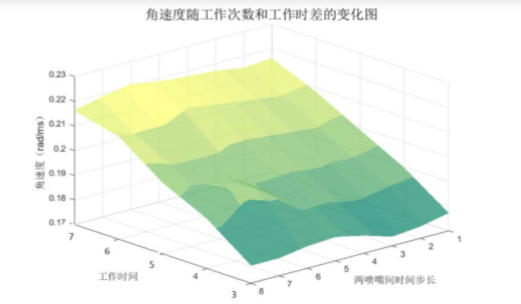
\includegraphics[width=12cm]{tu15.png} 
	
	\caption{角速度、工作次数和工作时差的变化规律 } \label{fig:15}
\end{figure}  

观察图\ref{fig:15}可以看出,当喷油器的工作次数恒定时,两喷油器起始工作时差对高压 油泵凸轮的角速度影响不大,然而当工作时差恒定时,凸轮转动的角速度随喷油器工作 次数的的增多而逐渐减小。

2)确定高压油泵和减压阀的控制模型下两个参数$\mu,\omega$对应的值为: 

利用 MATLAB 软件画出单向减压阀的开放总时间$\mu$随凸轮角速度$\omega$的变化曲线如
下图\ref{fig:16}所示: 
 \begin{figure}[htb] \centering 
	
	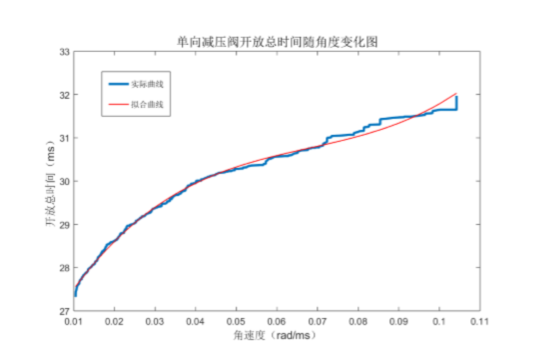
\includegraphics[width=12cm]{tu16.png} 
	
	\caption{单向减压阀的开放总时间随角速度的变化曲线} \label{fig:16}
\end{figure}  


分析表 4,发现单向减压阀的开放总时间$\mu$随凸轮角速度$\omega$的增大,呈现上升趋势, 但增长率逐渐减小且符合实际,角速度的增大会增大单位时间内从高压油泵流入高压油管的进油量,从而导致高压油管内的压强增大,所以需要增加单向减压阀的开放时间, 有效地控制高压油管的压力保持在稳定值左右。 

观察图\ref{fig:16}可知,我们利用多项式拟合的方法,对求得的单向减压阀的开放总时间 与角速度的变化曲线进行拟合,得到拟合方程为: 
\begin{equation}
\mu\left(\omega\right)=10540\omega^{3}-2145\omega^{2}+166.5\omega+26.05\label{eq:29}
\end{equation}

该拟合方程的决定系数$R^{2}=0.9973=99.73\%$,表示该一元三次方程对变化曲线的拟 合度很高。

\section{模型的评价与推广}

\subsection{模型的优点}
1.问题一结合液压油路的建模原理建立了高压油管的压强控制模型,建立了压强与 燃油流量的关系式,该模型对不确定性参数进行处理,将复杂形式简单化易于模型求解, 并且从不同情形下分析高压油管内压强的状态变化,增强了模型的完整性。 

2.在问题一模型的求解过程中,本文以残差平方和最小为目标,计算出单向阀的开 启时长,然后利用 GA 优化算法求出最优的单向阀开启时长,跳出局部最优解的限制, 遍历求得全局最优解。 

3.在问题二的模型建立中,针对高压油泵压油与喷油嘴出油,建立高压油泵模型与 喷油器模型对进油量与出油量进行控制,再结合问题一的高压油管压强控制模型,将燃 油系统划分为三部分讨论,使模型的思路易懂,条理清晰。 

\subsection{模型的缺点 }
本文在分析高压油泵模型时,为了简化模型,忽略高压油泵中柱塞和柱塞腔间间隙 漏油量以及压力波对燃油系统的影响,但在实际情况中柱塞上下运动会造成燃油泄漏, 从而影响高压油泵内的压力。

\subsection{模型的推广 }
\subsubsection{模型的应用}
高压油管压强控制模型被广泛应用于 GDI 发动机的轨压控制研究、GDI 燃油系统 研发平台、以及柴油机共轨压力模拟控制系统开发\textsuperscript{\cite{bib:two}}等方面。 


\subsubsection{模型的改进}
从实际情况出发,考虑高压油泵内燃油泄漏会对系统造成影响,在高压油泵压力状 态中的燃油泄漏量$q_{0}$与高压油泵柱塞升程有关,在柱塞泵油、柱塞上升时燃油泄漏量较 大,而柱塞下降时泄漏量较小,由此加入参数$q_{0}$,就使得高压油泵压力状态中包含了此 燃油泄漏的参数不确定性。从而得到燃油系统的模型为:
\begin{equation*}
\begin{cases}
\dot{p_{b}}=\frac{E}{V_{b}\left(\theta\right)}\left(A_{b}\cdot \omega_{gbm} \frac{dh_{b}}{d\theta}+U\cdot a_{11}\cdot \sqrt{p_{t}-p_{b}}-a_{12}\cdot\sqrt{p_{b}-p_{g}}-q_{0}\right)\\
\dot{p_{g}}=\frac{E}{V_{g}}\left(a_{12}\cdot\sqrt{p_{b}-p_{g}}-q_{gi}\right)\\
a_{11}=c_{tb}\cdot A_{tb}\cdot\sqrt{\frac{2}{\rho}}\\
a_{12}=c_{bg}\cdot A_{bg}\cdot\sqrt{\frac{2}{\rho}}
\end{cases}
\end{equation*} 

其中$p_{b}$为高压油泵内压强,$p_{g}$为高压油管内压强,$q_{gi}$ 为喷油速率,再对模型进行 符号函数与相关参数的化简,得到变换后的模型为: 

上式中U 表示压力调节阀的开关量,可以用-1 或 0 表示,令$u=U\cdot a_{11}\cdot\sqrt{P_{t}-p_{b}}$模 型改写为状态空间形式如下: 
\begin{equation*}
\begin{cases}
\dot{x_{1}}=\frac{E}{V_{b}\left(\theta\right)}\left(A_{b}\cdot\omega_{gbm}\frac{dh_{b}}{d\theta}+\mu-a_{12}\cdot\sqrt{x_{1}-x_{2}}-q_{0}\right)\\
\dot{x_{2}}==\frac{E}{V_{g}}\left(a_{12}\cdot\sqrt{x_{1}-x_{2}}-q_{gi}\right)
\end{cases}
\end{equation*}

基于上述模型可设计控制算法对其进行求解。 
%参考文献
\begin{thebibliography}{20}%宽度9
	\bibitem{bib:one}  Lee J C , Liu H , Noh Y J , et al. A Model Based Design Analysis for a Gasoline Direct Injection Pump[J]. 2015. 
	\bibitem{bib:two}欣白宇. GDI 发动机的轨压控制研究[D].吉林大学,2012. 
	\bibitem{bib:three}Lino P , Maione B , Rizzo A . Nonlinear modelling and control of a common rail injection system for diesel engines[J]. Applied Mathematical Modelling, 2007, 31(9):1770-1784.
	\bibitem{bib:four}康睿. 共轨喷油器仿真计算及参数优化[D].中国地质大学(北京),2012. 
	\bibitem{bib:five}武玉琪. GDI 燃油系统研发平台的开发[D].山东大学,2019.
	\bibitem{bib:six}刘海波.基于凸轮驱动的高压柱塞泵问题研究[J].内燃机与配件,2019(08):82-84. 
	\bibitem{bib:seven}郭益友. 平行分度凸轮机构的凸轮曲线计算机辅助设计[J]. 机械设计与制造工程, 2004(11):92-93.
	\bibitem{bib:eight} 魏啟印,张洪涛,姜峰.共轨式高压油泵凸轮型线对柱塞腔油压的影响[J].广西工学院学 报,2012,23(04):47-50+55 
	\bibitem{bib:nine}孙永厚, 张宇轩, 黄美发, et al. 喷油嘴针阀的公差建模及规范设计[J]. 组合机床与 自动化加工技术, 2016(6):55-58.
	\bibitem{bib:ten}刘天翔. 高压共轨喷油器针阀运动的特性研究[D].北京工业大学,2018.
	\bibitem{bib:eleven}吕晓辰. 高压共轨系统高压管路压力波动特性仿真研究及结构优化[D].北京交通大 学,2016.
	\bibitem{bib:twelve}郝真真. 生物柴油喷射系统嘴端压力分析[D].广西科技大学,2015.
	\bibitem{bib:thirteen}张美娟. 柴油机共轨压力模拟控制系统开发[D].江南大学,2006
\end{thebibliography}


\newpage
%附录
\begin{appendices}
	\section{排队算法--matlab 源程序}
	\begin{lstlisting}[language=matlab]
	kk=2;[mdd,ndd]=size(dd);
	while ~isempty(V)
	[tmpd,j]=min(W(i,V));tmpj=V(j);
	for k=2:ndd
	[tmp1,jj]=min(dd(1,k)+W(dd(2,k),V));
	tmp2=V(jj);tt(k-1,:)=[tmp1,tmp2,jj];
	end
	tmp=[tmpd,tmpj,j;tt];[tmp3,tmp4]=min(tmp(:,1));
	if tmp3==tmpd, ss(1:2,kk)=[i;tmp(tmp4,2)];
	else,tmp5=find(ss(:,tmp4)~=0);tmp6=length(tmp5);
	if dd(2,tmp4)==ss(tmp6,tmp4)
	ss(1:tmp6+1,kk)=[ss(tmp5,tmp4);tmp(tmp4,2)];
	else, ss(1:3,kk)=[i;dd(2,tmp4);tmp(tmp4,2)];
	end;end
	dd=[dd,[tmp3;tmp(tmp4,2)]];V(tmp(tmp4,3))=[];
	[mdd,ndd]=size(dd);kk=kk+1;
	end; S=ss; D=dd(1,:);
	\end{lstlisting}
	\section{规划解决程序--lingo源代码}
	\begin{lstlisting}[language=c]
	kk=2;
	[mdd,ndd]=size(dd);
	while ~isempty(V)
	[tmpd,j]=min(W(i,V));tmpj=V(j);
	for k=2:ndd
	[tmp1,jj]=min(dd(1,k)+W(dd(2,k),V));
	tmp2=V(jj);tt(k-1,:)=[tmp1,tmp2,jj];
	end
	tmp=[tmpd,tmpj,j;tt];[tmp3,tmp4]=min(tmp(:,1));
	if tmp3==tmpd, ss(1:2,kk)=[i;tmp(tmp4,2)];
	else,tmp5=find(ss(:,tmp4)~=0);tmp6=length(tmp5);
	if dd(2,tmp4)==ss(tmp6,tmp4)
	ss(1:tmp6+1,kk)=[ss(tmp5,tmp4);tmp(tmp4,2)];
	else, ss(1:3,kk)=[i;dd(2,tmp4);tmp(tmp4,2)];
	end;
	end
	dd=[dd,[tmp3;tmp(tmp4,2)]];V(tmp(tmp4,3))=[];
	[mdd,ndd]=size(dd);
	kk=kk+1;
	end;
	S=ss;
	D=dd(1,:);
	\end{lstlisting}
\end{appendices}

\end{document}